% algemene structuur:
%
% - wat is CHR?
% - CCHR: doelstellingen
% - taal
% - impl
% - bench


\documentclass{beamer}

\mode<article>
{
  \usepackage{fullpage}
  \usepackage{hyperref}
}

\mode<presentation>
{
  \usepackage{hyperref}
  \setbeamertemplate{background canvas}[vertical shading][bottom=white!10,top=blue!10]
  \usetheme{Warsaw}
%  \usefonttheme[onlysmall]{structurebold}
}

\usepackage{amsmath}
\usepackage{pstricks}
\usepackage{listings}
\usepackage{color}
\usepackage[dutch]{babel}
\usepackage{fancyvrb}
\usepackage{ulem}

\setbeamertemplate{example text}{Voorbeeld}
\renewcommand{\emph}[1]{\textit{{#1}}}
\definecolor{dgreen}{rgb}{0,0.7,0}
\definecolor{dbrown}{rgb}{0.4,0.3,0.1}
\definecolor{dred}{rgb}{0.5,0,0}
\newcommand{\bs}{$\backslash$}
\newcommand{\cConstr}[1]{\textcolor{blue}{#1}}
\newcommand{\cMacro}[1]{\textcolor{dred}{#1}}
\newcommand{\cComment}[1]{\textcolor{dgreen}{#1}}
\newcommand{\cLogic}[1]{\textcolor{black}{#1}}
\newcommand{\cFront}[1]{\textcolor{black}{#1}}
\newcommand{\cKey}[1]{\textcolor{red}{#1}}
\newcommand{\code}[1]{{\tt #1}}

\setbeamercolor{background canvas}{bg=white}
\setbeamertemplate{footline}[frame number]
\setbeamertemplate{navigation symbols}{}

\title{CCHR: De snelste CHR implementatie}
\subtitle{Pieter Wuille}

\author{Promotor: \\
Prof. Dr. Bart Demoen \\
Begeleider: \\
Dr. ir. Tom Schrijvers}

\date{29 mei 2007}

\begin{document}

\frame{\titlepage}


\begin{frame}
  \frametitle{Overzicht}
  \tableofcontents[hideothersubsections]
\end{frame}

\AtBeginSection[]
{
  \begin{frame}<beamer>
    \frametitle{Overzicht}
    \tableofcontents[currentsection,currentsection,hideothersubsections]
  \end{frame}
}

\section{Inleiding}

\subsection{Wat is CHR?}

\begin{frame}[containsverbatim]
  \frametitle{CHR}
  \begin{block}{Wat is CHR?}
    \begin{itemize}
      \item Een hoog-niveau declaratieve taaluitbreiding (van gasttaal)
      \item Regelgebaseerde omzetting van CHR constraints naar \begin{itemize}
        \item Andere CHR constraints
        \item Built-in constraints (door gasttaal aangeboden)
      \end{itemize}
      \item In feite multiset herschrijfregels
    \end{itemize}
  \end{block}

\end{frame}

\subsection{Voorbeelden}

\begin{frame}[containsverbatim]
  \frametitle{CHR syntax}
  \begin{example}{Grootst gemene deler in CHR(Prolog)}
\begin{Verbatim}[commandchars=\\\{\}]
:- \cKey{chr_constraint} \cConstr{prime}(+int), \cConstr{upto}(+natural)\cKey{.}

\cConstr{upto}(X) \cKey{<=>} X<2 \cKey{|} \cKey{true}\cKey{.}
\cConstr{upto}(X) \cKey{==>} X>1 \cKey{|} Y is X-1, \cConstr{upto}(Y), \cConstr{prime}(X)\cKey{.}
\cConstr{prime}(X) \cKey{\bs} \cConstr{prime}(Y) \cKey{<=>} Z is Y mod X, Z==0 \cKey{|} true\cKey{.}
\end{Verbatim}
  \end{example}

  \begin{block}{CHR Syntax}
    \begin{itemize}
      \item Regels voor herschrijven CHR constraint store
      \item Simplification, propagation en simpagation regels \begin{itemize}
        \item Simplification: {Rem} \code{<=>} {Guard} \code{|} {Body}
        \item Propagation: {Kept} \code{==>} {Guard} \code{|} {Body}
        \item Simpagation: {Kept} \bs {Rem} \code{<=>} {Guard} \code{|} {Body}
      \end{itemize}
    \end{itemize}
  \end{block}
\end{frame}

\subsection{Doelstellingen}

\begin{frame}
  \frametitle{Doelstellingen CCHR}
  \begin{block}{Doelstellingen}
    \begin{itemize}
      \item Een zo effici\"ent mogelijke CHR implementatie schrijven
      \item C als gasttaal gebruiken
    \end{itemize}
  \end{block}

  \begin{block}{Mogelijkheden C}
    \begin{itemize}
      \item Veel vrijheid datastructuren
      \item Directe geheugentoegang
      \item Bestaande optimaliserende compilers
      \item Bindings in veel andere talen
    \end{itemize}
  \end{block}

\end{frame}

\section{De taal}

\subsection{Syntax}

\begin{frame}
  \frametitle{CCHR: De taal}
  \begin{block}{Syntax}
    \begin{itemize}
      \item Binnen een \code{cchr}-blok in C code
      \item Constraint declaraties (argumenten: meeste C types)
      \item Regels gelijkaardig aan CHR syntax
      \item Arbitraire C expressies en statements in guard en body
      \item Lokale variabelen in guard en body
      \item Logische variabelen zijn mogelijk
    \end{itemize}
  \end{block}
\end{frame}

\subsection{Voorbeelden}

\begin{frame}[containsverbatim]
  \frametitle{CCHR: Voorbeeld 1}
  \begin{example}[Voorbeeld 1]{\tiny
\begin{Verbatim}[commandchars=\\\{\}]
\cMacro{#include <stdio.h>}
\cMacro{#include <stdlib.h>}

\cMacro{#include "fib_cchr.h"} \cComment{/* header gegenereerd door CCHR compiler */}

\cKey{cchr} \{
  \cKey{constraint} \cConstr{fib}(int,long),\cConstr{upto}(int)\cKey{;}

  begin \cKey{@} \cConstr{upto}(_) \cKey{==>} \cConstr{fib}(0,1L), \cConstr{fib}(1,1L)\cKey{;}
  calc \cKey{@}  \cConstr{upto}(Max), \cConstr{fib}(N2,M2) \cKey{\bs} \cConstr{fib}(N1,M1) \cKey{<=>} \cKey{alt}(N2==N1+1,N2-1==N1), N2<Max \cKey{|}
              \cConstr{fib}(N2+1, M1+M2)\cKey{;}
\}

int main(int argc, char **argv) \{
  cchr_runtime_init();
  cchr_add_\cConstr{upto}_1(90); \cComment{/* voeg upto(90) toe */}
  cchr_consloop(j,\cConstr{fib}_2,\{
    printf("fib(%i,%li){\bs}n",cchr_consarg(j,\cConstr{fib}_2,1),(long)cchr_consarg(j,\cConstr{fib}_2,2));
  \});
  cchr_runtime_free();
  return 0;
\}
\end{Verbatim}
}  \end{example}
\end{frame}


\begin{frame}[containsverbatim]
  \frametitle{CCHR: Voorbeeld 2}
  \begin{example}[Voorbeeld 2]{\scriptsize
\begin{Verbatim}[commandchars=\\\{\}]
\cComment{/* definieer log_int_t als een logische variabele van int's */}
\cLogic{logical_header}(int,int,log_int_t)

\cComment{/* cchr blok */}
\cKey{cchr} \{
  \cKey{constraint} \cConstr{fib}(int,log_int_t)
          \cKey{option}(destr,\{\cLogic{log_int_t_destruct}($2);\})
          \cKey{option}(init,\{\cLogic{log_int_t_copy}($2);\})\cKey{;}

  dup \cKey{@} \cConstr{fib}(N,M1) \cKey{\bs} \cConstr{fib}(N,M2) \cKey{<=>} \{ \cLogic{log_int_t_seteq}(M1,M2); \}\cKey{;}
  f01 \cKey{@} \cConstr{fib}(N,M) \cKey{==>} N<2 \cKey{|} \{ \cLogic{log_int_t_setval}(M,1); \}\cKey{;}
  fn  \cKey{@} \cConstr{fib}(N,M) \cKey{==>} N>1 \cKey{|}
    log_int_t M1=\cLogic{log_int_t_create}(), log_int_t M2=\cLogic{log_int_t_create}(),
    \cConstr{fib}(N-2,M1), \cConstr{fib}(N-1,M2),
    \{ \cLogic{log_int_t_setval}(M,\cLogic{log_int_t_getval}(M1)+\cLogic{log_int_t_getval}(M2)); \},
    \{ \cLogic{log_int_t_destruct}(M1); \cLogic{log_int_t_destruct}(M2); \}\cKey{;}
\}
\end{Verbatim}
}
  \end{example}
\end{frame}

\section{Implementatie}

\subsection{Overzicht}

\begin{frame}[containsverbatim]
  \frametitle{Opbouw CCHR}
  \begin{columns}[c]
  \column{0.40\textwidth}
  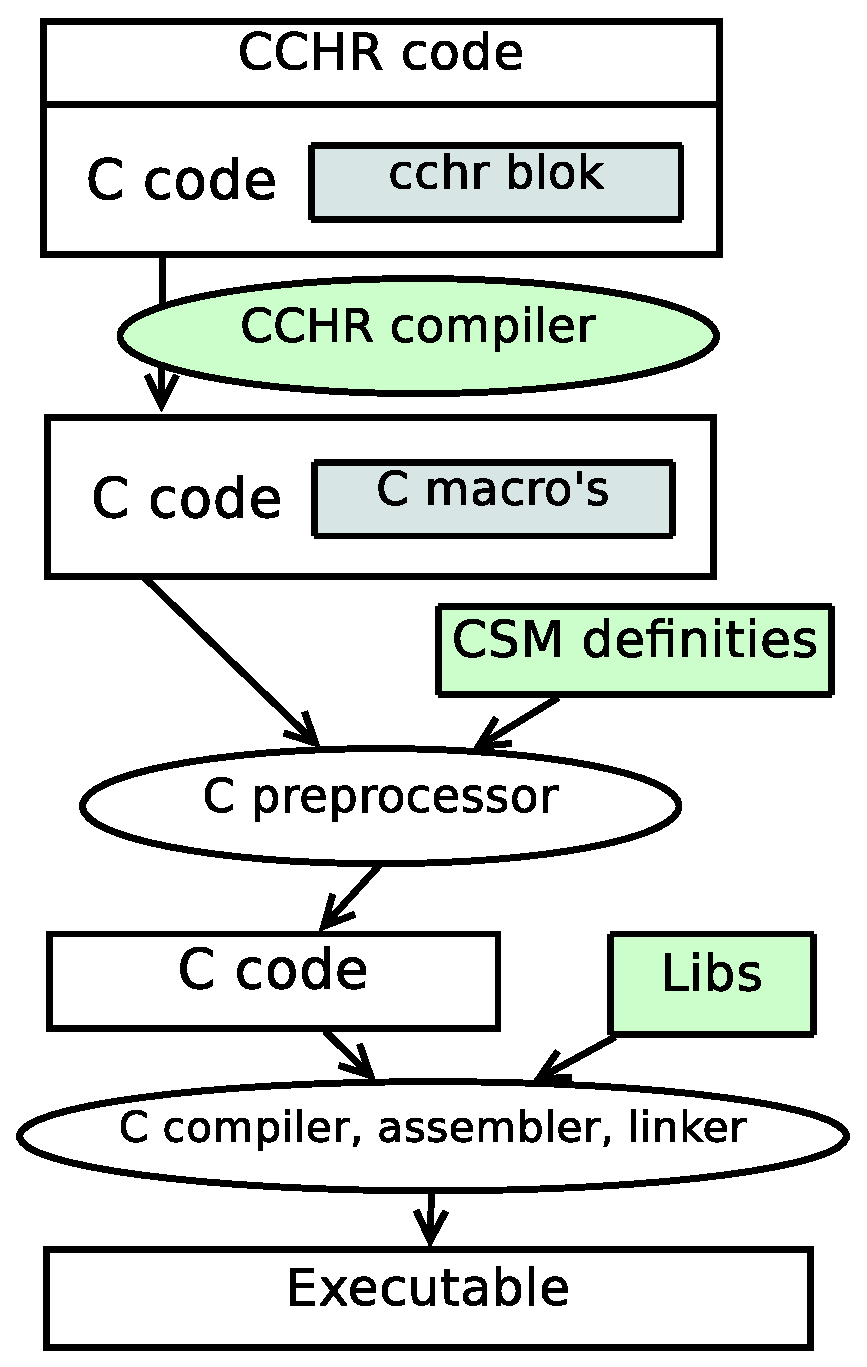
\includegraphics[height=0.83\textheight]{fig/overzicht}
  \column{0.60\textwidth}
  \begin{block}{Compilatieproces}
    \begin{itemize}
      \item CCHR code wordt door CCHR compiler doorlopen
      \item C code kopi\"eren, CCHR code vertalen naar macro's
      \item Gegenereerde code compileren (mbv. CSM definities)
      \item Extra libs (bv. code voor hashtable) compileren
      \item Samen linken tot executable
    \end{itemize}
    Het resultaat is een platform-specifiek, effici\"ent programma.
  \end{block}
  \end{columns}
\end{frame}

\subsection{CCHR Compiler}

\begin{frame}
  \frametitle{CCHR Compiler}
  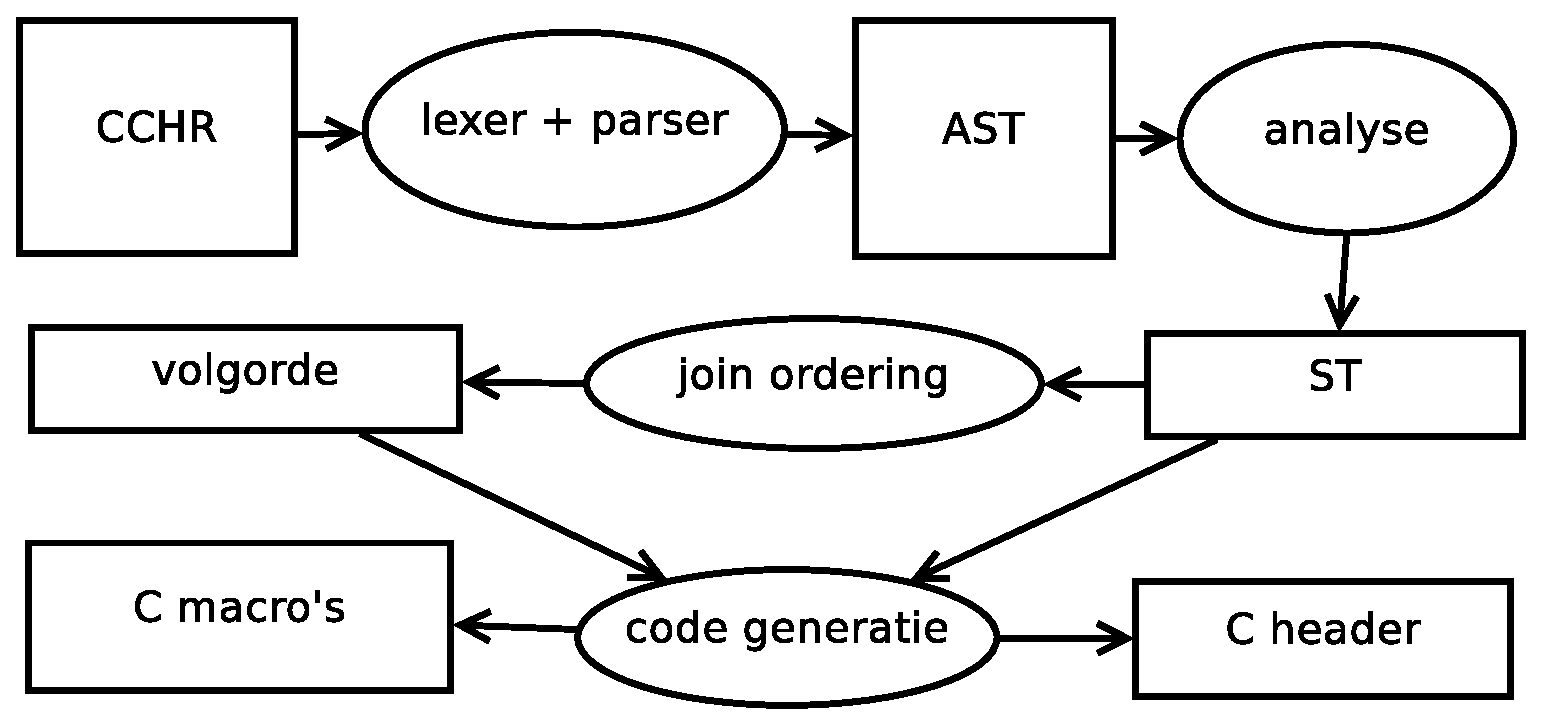
\includegraphics[width=1\textwidth]{fig/compil}
\end{frame}

\begin{frame}
  \frametitle{Lexer en Parser}
  \begin{block}{Lexer}
    \begin{itemize}
      \item Geschreven mbv. Flex, die lexer in C genereert.
      \item Splitst invoer in operatoren, haakjes, symbolen.
      \item Deze `tokens' worden aan parser gegeven.
    \end{itemize}
  \end{block}
  \begin{block}{Parser}
    \begin{itemize}
      \item Geschreven mbv. Bison, die parser in C genereert.
      \item Herkent regels, code-blokken, argumenten, constraints, \ldots
      \item Bouwt Abstract Syntax Tree (AST)
    \end{itemize}
  \end{block}
\end{frame}

\begin{frame}
  \frametitle{Analyse}
  \begin{block}{Analyse}
    Tijdens de analyse wordt de AST omgezet in een tussenvorm (semantic tree, ST)
    \begin{itemize}
      \item Alle types, variabelen, constraints, rules, occurrences worden objecten met
            onderlinge verwijzingen ipv. strings.
      \item Alle regels zijn omgezet naar Head Normal Form (HNF).
      \item Onderlinge afhankelijkheden tussen variabelen en occurrences worden bepaald.
    \end{itemize}
  \end{block}
\end{frame}

\begin{frame}
  \frametitle{Join ordering en code generatie}
  \begin{block}{Join ordering}
    Voor elke constraint occurrence moet iteratievolgorde en -methode bepaald worden
    voor elke partner constraint.
    \begin{itemize}
      \item Alle mogelijke volgordes afgaan.
      \item Gewicht toekennen aan elke volgorde.
      \item Volgorde met laagste gewicht kiezen.
      \item Guard met iterator combineren (index).
    \end{itemize}
  \end{block}
  \begin{block}{Code generatie}
    C macro's en een C header genereren voor elke:
    \begin{itemize}
      \item constraint, constraint occurrence, rule
      \item index, propagation geschiedenis, \ldots
    \end{itemize}
  \end{block}
\end{frame}

\subsection{Gegenereerde code}
\frame[containsverbatim]{\frametitle{Voorbeeld - CCHR code}
  \begin{example}
  \begin{Verbatim}[commandchars=\\\{\}]
\cKey{constraint} \cConstr{fib}(int,long),\cConstr{upto}(int)\cKey{;}

begin \cKey{@} \cConstr{upto}(_) ==> \cConstr{upto}(0,1L), \cConstr{upto}(1,1L)\cKey{;}
calc \cKey{@}  \cConstr{upto}(Max), \cConstr{fib}(N2,M2) \bs {\em \cConstr{fib}(N1,M1)}
        \cKey{<=>} \cKey{alt}(N2==N1+1,N2-1==N1), N2<Max
        \cKey{|} \cConstr{fib}(N2+1, M1+M2)\cKey{;}
  \end{Verbatim}
  \end{example}
}
\frame[containsverbatim]{\frametitle{Voorbeeld - C Macro's}
  \begin{example}[generated code]
  {\scriptsize \begin{Verbatim}[commandchars=\\\{\}]
#define CODELIST_\cConstr{fib}_2_calc_R1 {\bs}
  \cKey{CSM_IMMLOCAL}(int,N1,\cKey{CSM_ARG}(\cConstr{fib}_2,arg1)) {\bs}
  \cKey{CSM_IMMLOCAL}(long,M1,\cKey{CSM_ARG}(\cConstr{fib}_2,arg2)) {\bs}
  \cKey{CSM_DEFIDXVAR}(\cConstr{fib}_2,idx1,K2) {\bs}
  \cKey{CSM_SETIDXVAR}(\cConstr{fib}_2,idx1,K2,arg1,\cKey{CSM_LOCAL}(N1) + 1) {\bs}
  \cKey{CSM_IDXLOOP}(\cConstr{fib}_2,idx1,K2, {\bs}
    \cKey{CSM_IF}(\cKey{CSM_DIFFSELF}(K2), {\bs}
      \cKey{CSM_IMMLOCAL}(int,N2,{CSM_LARG}(\cConstr{fib}_2,K2,arg1)) {\bs}
      \cKey{CSM_IMMLOCAL}(long,M2,{CSM_LARG}(\cConstr{fib}_2,K2,arg2)) {\bs}
      \cKey{CSM_LOOP}(\cConstr{upto}_1,K1, {\bs}
        \cKey{CSM_IMMLOCAL}(int,Max,{CSM_LARG}(\cConstr{upto}_1,K1,arg1)) {\bs}
        \cKey{CSM_IF}(\cKey{CSM_LOCAL}(N2) < \cKey{CSM_LOCAL}(Max), {\bs}
          \cKey{CSM_KILLSELF}(\cConstr{fib}_2) {\bs}
          \cKey{CSM_ADD}(\cConstr{fib}_2,\cKey{CSM_LOCAL}(N2)+1,\cKey{CSM_LOCAL}(M1)+\cKey{CSM_LOCAL}(M2)) {\bs}
          \cKey{CSM_END} {\bs}
        ) {\bs}
      ) {\bs}
    ) {\bs}
  )
\end{Verbatim}
  }\end{example}
}

\subsection{Overige code}

\begin{frame}
  \frametitle{CSM definities}
  \begin{block}{CSM definities}
    \begin{itemize}
      \item Schermen implementatie-details af van codegenerator.
      \item Datastructuren kunnen gewijzigd worden zonder codegenerator aan te passen.
      \item Definieert de \code{CSM\_START} macro.
      \item Gedefinieerd in bestand \code{cchr\_csm.h}, dat in gegenereerde header ingeladen wordt.
    \end{itemize}
  \end{block}
\end{frame}

\begin{frame}
  \frametitle{Hashtables}
  \begin{block}{Hashtable}
    \begin{itemize}
      \item Datastructuur om in $O(1)$ tijd elementen op te zoeken.
      \item Zelf ge\"implementeerd Cuckoo-hashing algoritme.
      \item Gebruikt om indexen en propagation geschiedenis in bij te houden.
    \end{itemize}
  \end{block}
  \begin{block}{Hashfunctie}
    \begin{itemize}
      \item Hashtable vereist grillige functie om elementen op getallen af te beelden.
      \item Het public-domain lookup3 algoritme gebruikt.
    \end{itemize}
  \end{block}
\end{frame}

\begin{frame}
  \frametitle{Logische variabelen}
  \begin{block}{Logische variabelen}
    \begin{itemize}
      \item Variabelen die een waarde kunnen hebben of niet
      \item Waarover onderlinge gelijkheden bekend kunnen zijn
      \item Ge\"implementeerd met een C implementatie van het
            Union-Find algoritme
      \item Ook buiten CCHR bruikbaar
    \end{itemize}
  \end{block}
\end{frame}

\section{Benchmarks}

\subsection{Fibonacci}

\begin{frame}
  \frametitle{Benchmark: Fibonacci}
  \includegraphics[width=\textwidth]{fig/bench-fib}
\end{frame}

\subsection{Kleiner-dan of gelijk-aan}

\begin{frame}
  \frametitle{Benchmark: Kleiner-dan of gelijk-aan}
  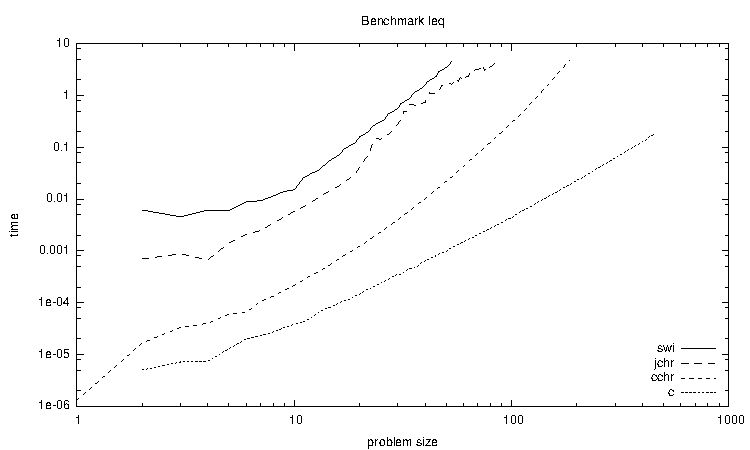
\includegraphics[width=\textwidth]{fig/bench-leq}
\end{frame}

\subsection{Grootste gemene deler}

\begin{frame}
  \frametitle{Benchmark: Grootste gemene deler}
  \includegraphics[width=\textwidth]{fig/bench-gcd}
\end{frame}

\subsection{Vergelijking}

\begin{frame}
\frametitle{Vergelijking benchmarks}
\begin{center}
\cFront{\begin{tabular}{|c|rrr@{.}lr|}
\hline
 & {\bf SWI} & {\bf JCHR} & \multicolumn{2}{c}{\bf CCHR} & {\bf C} \\
\hline
gcd    & 22000 & -     &   3&4  & 1 \\
fib    & 21000 & 940   &   8&5  & 1 \\
primes & 310   & 490   &   6&9  & 1 \\
tak    & 210   & 110   &   4&3  & 1 \\
leq    & 1100  & 440   &   9&8  & 1 \\
ram    & 4700  & 11000 &  120&0 & 1 \\
\hline
\end{tabular}}
\end{center}
\end{frame}

\section{Conclusie}

\begin{frame}
  \frametitle{Conclusie}
  \begin{block}{Conclusie}
    Met deze thesis is aangetoond dat:
    \begin{itemize}
      \item Een CHR implementatie in/voor C mogelijk is
      \item en dat het een snelheidswinst oplevert
    \end{itemize}
  \end{block}
\end{frame}

\begin{frame}
  \frametitle{Einde}
  \cFront{Einde}
\end{frame}

\end{document}

